\documentclass[1p]{elsarticle_modified}
%\bibliographystyle{elsarticle-num}

%\usepackage[colorlinks]{hyperref}
%\usepackage{abbrmath_seonhwa} %\Abb, \Ascr, \Acal ,\Abf, \Afrak
\usepackage{amsfonts}
\usepackage{amssymb}
\usepackage{amsmath}
\usepackage{amsthm}
\usepackage{scalefnt}
\usepackage{amsbsy}
\usepackage{kotex}
\usepackage{caption}
\usepackage{subfig}
\usepackage{color}
\usepackage{graphicx}
\usepackage{xcolor} %% white, black, red, green, blue, cyan, magenta, yellow
\usepackage{float}
\usepackage{setspace}
\usepackage{hyperref}

\usepackage{tikz}
\usetikzlibrary{arrows}

\usepackage{multirow}
\usepackage{array} % fixed length table
\usepackage{hhline}

%%%%%%%%%%%%%%%%%%%%%
\makeatletter
\renewcommand*\env@matrix[1][\arraystretch]{%
	\edef\arraystretch{#1}%
	\hskip -\arraycolsep
	\let\@ifnextchar\new@ifnextchar
	\array{*\c@MaxMatrixCols c}}
\makeatother %https://tex.stackexchange.com/questions/14071/how-can-i-increase-the-line-spacing-in-a-matrix
%%%%%%%%%%%%%%%

\usepackage[normalem]{ulem}

\newcommand{\msout}[1]{\ifmmode\text{\sout{\ensuremath{#1}}}\else\sout{#1}\fi}
%SOURCE: \msout is \stkout macro in https://tex.stackexchange.com/questions/20609/strikeout-in-math-mode

\newcommand{\cancel}[1]{
	\ifmmode
	{\color{red}\msout{#1}}
	\else
	{\color{red}\sout{#1}}
	\fi
}

\newcommand{\add}[1]{
	{\color{blue}\uwave{#1}}
}

\newcommand{\replace}[2]{
	\ifmmode
	{\color{red}\msout{#1}}{\color{blue}\uwave{#2}}
	\else
	{\color{red}\sout{#1}}{\color{blue}\uwave{#2}}
	\fi
}

\newcommand{\Sol}{\mathcal{S}} %segment
\newcommand{\D}{D} %diagram
\newcommand{\A}{\mathcal{A}} %arc


%%%%%%%%%%%%%%%%%%%%%%%%%%%%%5 test

\def\sl{\operatorname{\textup{SL}}(2,\Cbb)}
\def\psl{\operatorname{\textup{PSL}}(2,\Cbb)}
\def\quan{\mkern 1mu \triangleright \mkern 1mu}

\theoremstyle{definition}
\newtheorem{thm}{Theorem}[section]
\newtheorem{prop}[thm]{Proposition}
\newtheorem{lem}[thm]{Lemma}
\newtheorem{ques}[thm]{Question}
\newtheorem{cor}[thm]{Corollary}
\newtheorem{defn}[thm]{Definition}
\newtheorem{exam}[thm]{Example}
\newtheorem{rmk}[thm]{Remark}
\newtheorem{alg}[thm]{Algorithm}

\newcommand{\I}{\sqrt{-1}}
\begin{document}

%\begin{frontmatter}
%
%\title{Boundary parabolic representations of knots up to 8 crossings}
%
%%% Group authors per affiliation:
%\author{Yunhi Cho} 
%\address{Department of Mathematics, University of Seoul, Seoul, Korea}
%\ead{yhcho@uos.ac.kr}
%
%
%\author{Seonhwa Kim} %\fnref{s_kim}}
%\address{Center for Geometry and Physics, Institute for Basic Science, Pohang, 37673, Korea}
%\ead{ryeona17@ibs.re.kr}
%
%\author{Hyuk Kim}
%\address{Department of Mathematical Sciences, Seoul National University, Seoul 08826, Korea}
%\ead{hyukkim@snu.ac.kr}
%
%\author{Seokbeom Yoon}
%\address{Department of Mathematical Sciences, Seoul National University, Seoul, 08826,  Korea}
%\ead{sbyoon15@snu.ac.kr}
%
%\begin{abstract}
%We find all boundary parabolic representation of knots up to 8 crossings.
%
%\end{abstract}
%\begin{keyword}
%    \MSC[2010] 57M25 
%\end{keyword}
%
%\end{frontmatter}

%\linenumbers
%\tableofcontents
%
\newcommand\colored[1]{\textcolor{white}{\rule[-0.35ex]{0.8em}{1.4ex}}\kern-0.8em\color{red} #1}%
%\newcommand\colored[1]{\textcolor{white}{ #1}\kern-2.17ex	\textcolor{white}{ #1}\kern-1.81ex	\textcolor{white}{ #1}\kern-2.15ex\color{red}#1	}

{\Large $\underline{12a_{0137}~(K12a_{0137})}$}

\setlength{\tabcolsep}{10pt}
\renewcommand{\arraystretch}{1.6}
\vspace{1cm}\begin{tabular}{m{100pt}>{\centering\arraybackslash}m{274pt}}
\multirow{5}{120pt}{
	\centering
	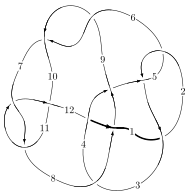
\includegraphics[width=112pt]{../../../GIT/diagram.site/Diagrams/png/938_12a_0137.png}\\
\ \ \ A knot diagram\footnotemark}&
\allowdisplaybreaks
\textbf{Linearized knot diagam} \\
\cline{2-2}
 &
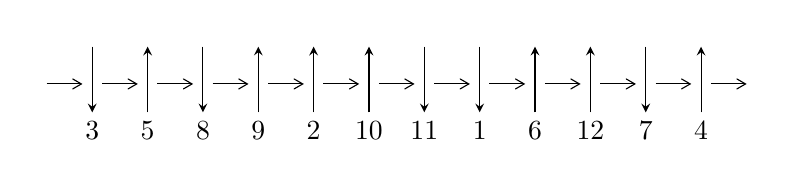
\begin{tikzpicture}[x=20pt, y=17pt]
	% nodes
	\node (C0) at (0, 0) {};
	\node (C1) at (1, 0) {};
	\node (C1U) at (1, +1) {};
	\node (C1D) at (1, -1) {3};

	\node (C2) at (2, 0) {};
	\node (C2U) at (2, +1) {};
	\node (C2D) at (2, -1) {5};

	\node (C3) at (3, 0) {};
	\node (C3U) at (3, +1) {};
	\node (C3D) at (3, -1) {8};

	\node (C4) at (4, 0) {};
	\node (C4U) at (4, +1) {};
	\node (C4D) at (4, -1) {9};

	\node (C5) at (5, 0) {};
	\node (C5U) at (5, +1) {};
	\node (C5D) at (5, -1) {2};

	\node (C6) at (6, 0) {};
	\node (C6U) at (6, +1) {};
	\node (C6D) at (6, -1) {10};

	\node (C7) at (7, 0) {};
	\node (C7U) at (7, +1) {};
	\node (C7D) at (7, -1) {11};

	\node (C8) at (8, 0) {};
	\node (C8U) at (8, +1) {};
	\node (C8D) at (8, -1) {1};

	\node (C9) at (9, 0) {};
	\node (C9U) at (9, +1) {};
	\node (C9D) at (9, -1) {6};

	\node (C10) at (10, 0) {};
	\node (C10U) at (10, +1) {};
	\node (C10D) at (10, -1) {12};

	\node (C11) at (11, 0) {};
	\node (C11U) at (11, +1) {};
	\node (C11D) at (11, -1) {7};

	\node (C12) at (12, 0) {};
	\node (C12U) at (12, +1) {};
	\node (C12D) at (12, -1) {4};
	\node (C13) at (13, 0) {};

	% arrows
	\draw[->,>={angle 60}]
	(C0) edge (C1) (C1) edge (C2) (C2) edge (C3) (C3) edge (C4) (C4) edge (C5) (C5) edge (C6) (C6) edge (C7) (C7) edge (C8) (C8) edge (C9) (C9) edge (C10) (C10) edge (C11) (C11) edge (C12) (C12) edge (C13) ;	\draw[->,>=stealth]
	(C1U) edge (C1D) (C2D) edge (C2U) (C3U) edge (C3D) (C4D) edge (C4U) (C5D) edge (C5U) (C6D) edge (C6U) (C7U) edge (C7D) (C8U) edge (C8D) (C9D) edge (C9U) (C10D) edge (C10U) (C11U) edge (C11D) (C12D) edge (C12U) ;
	\end{tikzpicture} \\
\hhline{~~} \\& 
\textbf{Solving Sequence} \\ \cline{2-2} 
 &
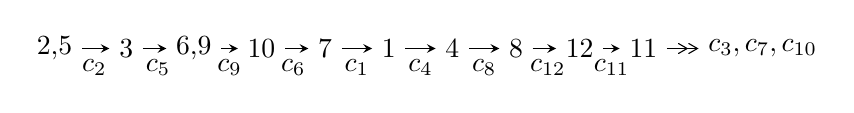
\begin{tikzpicture}[x=23pt, y=7pt]
	% node
	\node (A0) at (-1/8, 0) {2,5};
	\node (A1) at (1, 0) {3};
	\node (A2) at (33/16, 0) {6,9};
	\node (A3) at (25/8, 0) {10};
	\node (A4) at (33/8, 0) {7};
	\node (A5) at (41/8, 0) {1};
	\node (A6) at (49/8, 0) {4};
	\node (A7) at (57/8, 0) {8};
	\node (A8) at (65/8, 0) {12};
	\node (A9) at (73/8, 0) {11};
	\node (C1) at (1/2, -1) {$c_{2}$};
	\node (C2) at (3/2, -1) {$c_{5}$};
	\node (C3) at (21/8, -1) {$c_{9}$};
	\node (C4) at (29/8, -1) {$c_{6}$};
	\node (C5) at (37/8, -1) {$c_{1}$};
	\node (C6) at (45/8, -1) {$c_{4}$};
	\node (C7) at (53/8, -1) {$c_{8}$};
	\node (C8) at (61/8, -1) {$c_{12}$};
	\node (C9) at (69/8, -1) {$c_{11}$};
	\node (A10) at (11, 0) {$c_{3},c_{7},c_{10}$};

	% edge
	\draw[->,>=stealth]	
	(A0) edge (A1) (A1) edge (A2) (A2) edge (A3) (A3) edge (A4) (A4) edge (A5) (A5) edge (A6) (A6) edge (A7) (A7) edge (A8) (A8) edge (A9) ;
	\draw[->>,>={angle 60}]	
	(A9) edge (A10);
\end{tikzpicture} \\ 

\end{tabular} \\

\footnotetext{
The image of knot diagram is generated by the software ``\textbf{Draw programme}" developed by Andrew Bartholomew(\url{http://www.layer8.co.uk/maths/draw/index.htm\#Running-draw}), where we modified some parts for our purpose(\url{https://github.com/CATsTAILs/LinksPainter}).
}\phantom \\ \newline 
\centering \textbf{Ideals for irreducible components\footnotemark of $X_{\text{par}}$} 
 
\begin{align*}
I^u_{1}&=\langle 
6.13816\times10^{191} u^{110}-1.13429\times10^{193} u^{109}+\cdots+2.24718\times10^{193} b-3.38769\times10^{193},\\
\phantom{I^u_{1}}&\phantom{= \langle  }-1.81134\times10^{193} u^{110}+6.26196\times10^{193} u^{109}+\cdots+2.24718\times10^{193} a+3.37392\times10^{193},\\
\phantom{I^u_{1}}&\phantom{= \langle  }u^{111}-3 u^{110}+\cdots-8 u+1\rangle \\
I^u_{2}&=\langle 
b-2,\;a-1,\;u^2+u+1\rangle \\
I^u_{3}&=\langle 
b+1,\;a+u+1,\;u^2+u+1\rangle \\
\\
\end{align*}
\raggedright * 3 irreducible components of $\dim_{\mathbb{C}}=0$, with total 115 representations.\\
\footnotetext{All coefficients of polynomials are rational numbers. But the coefficients are sometimes approximated in decimal forms when there is not enough margin.}
\newpage
\renewcommand{\arraystretch}{1}
\centering \section*{I. $I^u_{1}= \langle 6.14\times10^{191} u^{110}-1.13\times10^{193} u^{109}+\cdots+2.25\times10^{193} b-3.39\times10^{193},\;-1.81\times10^{193} u^{110}+6.26\times10^{193} u^{109}+\cdots+2.25\times10^{193} a+3.37\times10^{193},\;u^{111}-3 u^{110}+\cdots-8 u+1 \rangle$}
\flushleft \textbf{(i) Arc colorings}\\
\begin{tabular}{m{7pt} m{180pt} m{7pt} m{180pt} }
\flushright $a_{2}=$&$\begin{pmatrix}1\\0\end{pmatrix}$ \\
\flushright $a_{5}=$&$\begin{pmatrix}0\\u\end{pmatrix}$ \\
\flushright $a_{3}=$&$\begin{pmatrix}1\\- u^2\end{pmatrix}$ \\
\flushright $a_{6}=$&$\begin{pmatrix}u\\u\end{pmatrix}$ \\
\flushright $a_{9}=$&$\begin{pmatrix}0.806049 u^{110}-2.78659 u^{109}+\cdots+32.2491 u-1.50140\\-0.0273149 u^{110}+0.504759 u^{109}+\cdots-8.15785 u+1.50753\end{pmatrix}$ \\
\flushright $a_{10}=$&$\begin{pmatrix}1.23473 u^{110}-4.63145 u^{109}+\cdots+39.4124 u-2.29265\\0.401363 u^{110}-1.34010 u^{109}+\cdots-0.994453 u+0.716275\end{pmatrix}$ \\
\flushright $a_{7}=$&$\begin{pmatrix}-0.344800 u^{110}+2.01151 u^{109}+\cdots-9.75297 u-2.65220\\-0.941826 u^{110}+2.82073 u^{109}+\cdots-2.64014 u+0.726247\end{pmatrix}$ \\
\flushright $a_{1}=$&$\begin{pmatrix}u^2+1\\- u^4\end{pmatrix}$ \\
\flushright $a_{4}=$&$\begin{pmatrix}0.325295 u^{110}-1.05138 u^{109}+\cdots-0.0877722 u+3.79641\\0.344661 u^{110}-0.920101 u^{109}+\cdots-2.58288 u+0.162347\end{pmatrix}$ \\
\flushright $a_{8}=$&$\begin{pmatrix}1.04968 u^{110}-3.66787 u^{109}+\cdots+30.1172 u-0.718132\\0.479923 u^{110}-1.04472 u^{109}+\cdots-3.71313 u+0.942185\end{pmatrix}$ \\
\flushright $a_{12}=$&$\begin{pmatrix}-0.193835 u^{110}+0.246390 u^{109}+\cdots-8.59881 u+2.39820\\0.0697190 u^{110}-0.380589 u^{109}+\cdots+1.11872 u-0.310933\end{pmatrix}$ \\
\flushright $a_{11}=$&$\begin{pmatrix}1.30011 u^{110}-2.29710 u^{109}+\cdots+18.8682 u+0.678898\\-1.16327 u^{110}+3.92263 u^{109}+\cdots-19.1527 u+3.07306\end{pmatrix}$\\&\end{tabular}
\flushleft \textbf{(ii) Obstruction class $= -1$}\\~\\
\flushleft \textbf{(iii) Cusp Shapes $= 0.199727 u^{110}-1.12797 u^{109}+\cdots+25.1841 u-1.58105$}\\~\\
\newpage\renewcommand{\arraystretch}{1}
\flushleft \textbf{(iv) u-Polynomials at the component}\newline \\
\begin{tabular}{m{50pt}|m{274pt}}
Crossings & \hspace{64pt}u-Polynomials at each crossing \\
\hline $$\begin{aligned}c_{1}\end{aligned}$$&$\begin{aligned}
&u^{111}+41 u^{110}+\cdots-12 u-1
\end{aligned}$\\
\hline $$\begin{aligned}c_{2},c_{5}\end{aligned}$$&$\begin{aligned}
&u^{111}+3 u^{110}+\cdots-8 u-1
\end{aligned}$\\
\hline $$\begin{aligned}c_{3}\end{aligned}$$&$\begin{aligned}
&u^{111}-2 u^{110}+\cdots+128151 u-22181
\end{aligned}$\\
\hline $$\begin{aligned}c_{4}\end{aligned}$$&$\begin{aligned}
&u^{111}+39 u^{109}+\cdots-10571037 u-2188019
\end{aligned}$\\
\hline $$\begin{aligned}c_{6},c_{9}\end{aligned}$$&$\begin{aligned}
&u^{111}-3 u^{110}+\cdots+3962 u-1217
\end{aligned}$\\
\hline $$\begin{aligned}c_{7},c_{11}\end{aligned}$$&$\begin{aligned}
&u^{111}+3 u^{110}+\cdots+2 u-1
\end{aligned}$\\
\hline $$\begin{aligned}c_{8}\end{aligned}$$&$\begin{aligned}
&u^{111}+3 u^{110}+\cdots-2 u-1
\end{aligned}$\\
\hline $$\begin{aligned}c_{10}\end{aligned}$$&$\begin{aligned}
&u^{111}-61 u^{110}+\cdots-8 u+1
\end{aligned}$\\
\hline $$\begin{aligned}c_{12}\end{aligned}$$&$\begin{aligned}
&u^{111}+11 u^{110}+\cdots-16 u+16
\end{aligned}$\\
\hline
\end{tabular}\\~\\
\newpage\renewcommand{\arraystretch}{1}
\flushleft \textbf{(v) Riley Polynomials at the component}\newline \\
\begin{tabular}{m{50pt}|m{274pt}}
Crossings & \hspace{64pt}Riley Polynomials at each crossing \\
\hline $$\begin{aligned}c_{1}\end{aligned}$$&$\begin{aligned}
&y^{111}+61 y^{110}+\cdots-2780 y-1
\end{aligned}$\\
\hline $$\begin{aligned}c_{2},c_{5}\end{aligned}$$&$\begin{aligned}
&y^{111}+41 y^{110}+\cdots-12 y-1
\end{aligned}$\\
\hline $$\begin{aligned}c_{3}\end{aligned}$$&$\begin{aligned}
&y^{111}+150 y^{110}+\cdots-11615036801 y-491996761
\end{aligned}$\\
\hline $$\begin{aligned}c_{4}\end{aligned}$$&$\begin{aligned}
&y^{111}+78 y^{110}+\cdots+215220189102279 y-4787427144361
\end{aligned}$\\
\hline $$\begin{aligned}c_{6},c_{9}\end{aligned}$$&$\begin{aligned}
&y^{111}-99 y^{110}+\cdots-22891192 y-1481089
\end{aligned}$\\
\hline $$\begin{aligned}c_{7},c_{11}\end{aligned}$$&$\begin{aligned}
&y^{111}+61 y^{110}+\cdots-8 y-1
\end{aligned}$\\
\hline $$\begin{aligned}c_{8}\end{aligned}$$&$\begin{aligned}
&y^{111}+13 y^{110}+\cdots-8 y-1
\end{aligned}$\\
\hline $$\begin{aligned}c_{10}\end{aligned}$$&$\begin{aligned}
&y^{111}-19 y^{110}+\cdots+148 y-1
\end{aligned}$\\
\hline $$\begin{aligned}c_{12}\end{aligned}$$&$\begin{aligned}
&y^{111}-25 y^{110}+\cdots+6272 y-256
\end{aligned}$\\
\hline
\end{tabular}\\~\\
\newpage\flushleft \textbf{(vi) Complex Volumes and Cusp Shapes}
$$\begin{array}{c|c|c}  
\text{Solutions to }I^u_{1}& \I (\text{vol} + \sqrt{-1}CS) & \text{Cusp shape}\\
 \hline 
\begin{aligned}
u &= \phantom{-}0.151572 + 0.991463 I \\
a &= -0.888867 - 0.508229 I \\
b &= -1.66325 - 0.01061 I\end{aligned}
 & -3.59561 - 0.34680 I & \phantom{-0.000000 } 0 \\ \hline\begin{aligned}
u &= \phantom{-}0.151572 - 0.991463 I \\
a &= -0.888867 + 0.508229 I \\
b &= -1.66325 + 0.01061 I\end{aligned}
 & -3.59561 + 0.34680 I & \phantom{-0.000000 } 0 \\ \hline\begin{aligned}
u &= \phantom{-}0.258560 + 0.953606 I \\
a &= \phantom{-}0.820900 + 0.539762 I \\
b &= \phantom{-}1.79814 - 0.31279 I\end{aligned}
 & -1.60150 + 4.05760 I & \phantom{-0.000000 } 0 \\ \hline\begin{aligned}
u &= \phantom{-}0.258560 - 0.953606 I \\
a &= \phantom{-}0.820900 - 0.539762 I \\
b &= \phantom{-}1.79814 + 0.31279 I\end{aligned}
 & -1.60150 - 4.05760 I & \phantom{-0.000000 } 0 \\ \hline\begin{aligned}
u &= \phantom{-}0.700734 + 0.735786 I \\
a &= \phantom{-}0.388751 - 1.180800 I \\
b &= -0.545202 + 0.253821 I\end{aligned}
 & \phantom{-}9.12536 - 4.91085 I & \phantom{-0.000000 } 0 \\ \hline\begin{aligned}
u &= \phantom{-}0.700734 - 0.735786 I \\
a &= \phantom{-}0.388751 + 1.180800 I \\
b &= -0.545202 - 0.253821 I\end{aligned}
 & \phantom{-}9.12536 + 4.91085 I & \phantom{-0.000000 } 0 \\ \hline\begin{aligned}
u &= -0.452673 + 0.873202 I \\
a &= \phantom{-}2.34656 - 0.61539 I \\
b &= \phantom{-}2.78531 - 1.07755 I\end{aligned}
 & \phantom{-}0.001017 - 0.573653 I & \phantom{-0.000000 } 0 \\ \hline\begin{aligned}
u &= -0.452673 - 0.873202 I \\
a &= \phantom{-}2.34656 + 0.61539 I \\
b &= \phantom{-}2.78531 + 1.07755 I\end{aligned}
 & \phantom{-}0.001017 + 0.573653 I & \phantom{-0.000000 } 0 \\ \hline\begin{aligned}
u &= \phantom{-}0.574894 + 0.794669 I \\
a &= \phantom{-}0.401800 - 0.342049 I \\
b &= \phantom{-}1.84011 - 0.11929 I\end{aligned}
 & \phantom{-}0.66452 + 3.75930 I & \phantom{-0.000000 } 0 \\ \hline\begin{aligned}
u &= \phantom{-}0.574894 - 0.794669 I \\
a &= \phantom{-}0.401800 + 0.342049 I \\
b &= \phantom{-}1.84011 + 0.11929 I\end{aligned}
 & \phantom{-}0.66452 - 3.75930 I & \phantom{-0.000000 } 0\\
 \hline 
 \end{array}$$\newpage$$\begin{array}{c|c|c}  
\text{Solutions to }I^u_{1}& \I (\text{vol} + \sqrt{-1}CS) & \text{Cusp shape}\\
 \hline 
\begin{aligned}
u &= \phantom{-}0.762307 + 0.679648 I \\
a &= \phantom{-}0.596090 - 0.841569 I \\
b &= \phantom{-}0.707490 - 0.483429 I\end{aligned}
 & \phantom{-}5.76477 - 1.56136 I & \phantom{-0.000000 } 0 \\ \hline\begin{aligned}
u &= \phantom{-}0.762307 - 0.679648 I \\
a &= \phantom{-}0.596090 + 0.841569 I \\
b &= \phantom{-}0.707490 + 0.483429 I\end{aligned}
 & \phantom{-}5.76477 + 1.56136 I & \phantom{-0.000000 } 0 \\ \hline\begin{aligned}
u &= -0.503793 + 0.893374 I \\
a &= -2.95406 + 1.43653 I \\
b &= -3.62966 + 1.39140 I\end{aligned}
 & \phantom{-}0.29861 - 3.79341 I & \phantom{-0.000000 } 0 \\ \hline\begin{aligned}
u &= -0.503793 - 0.893374 I \\
a &= -2.95406 - 1.43653 I \\
b &= -3.62966 - 1.39140 I\end{aligned}
 & \phantom{-}0.29861 + 3.79341 I & \phantom{-0.000000 } 0 \\ \hline\begin{aligned}
u &= \phantom{-}0.682390 + 0.771033 I \\
a &= -0.408080 + 1.072650 I \\
b &= \phantom{-}0.360693 - 0.288234 I\end{aligned}
 & \phantom{-}5.68044 + 0.15489 I & \phantom{-0.000000 } 0 \\ \hline\begin{aligned}
u &= \phantom{-}0.682390 - 0.771033 I \\
a &= -0.408080 - 1.072650 I \\
b &= \phantom{-}0.360693 + 0.288234 I\end{aligned}
 & \phantom{-}5.68044 - 0.15489 I & \phantom{-0.000000 } 0 \\ \hline\begin{aligned}
u &= -0.591641 + 0.849125 I \\
a &= \phantom{-}2.80917 - 1.82162 I \\
b &= \phantom{-}3.46325 - 0.58936 I\end{aligned}
 & \phantom{-}6.39356 + 2.13485 I & \phantom{-0.000000 } 0 \\ \hline\begin{aligned}
u &= -0.591641 - 0.849125 I \\
a &= \phantom{-}2.80917 + 1.82162 I \\
b &= \phantom{-}3.46325 + 0.58936 I\end{aligned}
 & \phantom{-}6.39356 - 2.13485 I & \phantom{-0.000000 } 0 \\ \hline\begin{aligned}
u &= -0.574926 + 0.863175 I \\
a &= -2.78033 + 1.84517 I \\
b &= -3.49720 + 0.84587 I\end{aligned}
 & \phantom{-}2.81370 - 2.28141 I & \phantom{-0.000000 } 0 \\ \hline\begin{aligned}
u &= -0.574926 - 0.863175 I \\
a &= -2.78033 - 1.84517 I \\
b &= -3.49720 - 0.84587 I\end{aligned}
 & \phantom{-}2.81370 + 2.28141 I & \phantom{-0.000000 } 0\\
 \hline 
 \end{array}$$\newpage$$\begin{array}{c|c|c}  
\text{Solutions to }I^u_{1}& \I (\text{vol} + \sqrt{-1}CS) & \text{Cusp shape}\\
 \hline 
\begin{aligned}
u &= \phantom{-}0.813992 + 0.499000 I \\
a &= \phantom{-}0.446497 - 1.221160 I \\
b &= \phantom{-}0.181652 + 0.047950 I\end{aligned}
 & \phantom{-}2.21997 - 7.60792 I & \phantom{-0.000000 } 0 \\ \hline\begin{aligned}
u &= \phantom{-}0.813992 - 0.499000 I \\
a &= \phantom{-}0.446497 + 1.221160 I \\
b &= \phantom{-}0.181652 - 0.047950 I\end{aligned}
 & \phantom{-}2.21997 + 7.60792 I & \phantom{-0.000000 } 0 \\ \hline\begin{aligned}
u &= -0.586237 + 0.879911 I \\
a &= \phantom{-}2.78417 - 1.86801 I \\
b &= \phantom{-}3.72891 - 0.83367 I\end{aligned}
 & \phantom{-}6.29471 - 6.78751 I & \phantom{-0.000000 } 0 \\ \hline\begin{aligned}
u &= -0.586237 - 0.879911 I \\
a &= \phantom{-}2.78417 + 1.86801 I \\
b &= \phantom{-}3.72891 + 0.83367 I\end{aligned}
 & \phantom{-}6.29471 + 6.78751 I & \phantom{-0.000000 } 0 \\ \hline\begin{aligned}
u &= -0.479587 + 0.810655 I \\
a &= -2.03914 + 1.62005 I \\
b &= -1.82668 + 1.01950 I\end{aligned}
 & \phantom{-}0.575579 - 0.242431 I & \phantom{-0.000000 } 0 \\ \hline\begin{aligned}
u &= -0.479587 - 0.810655 I \\
a &= -2.03914 - 1.62005 I \\
b &= -1.82668 - 1.01950 I\end{aligned}
 & \phantom{-}0.575579 + 0.242431 I & \phantom{-0.000000 } 0 \\ \hline\begin{aligned}
u &= \phantom{-}0.715946 + 0.802237 I \\
a &= \phantom{-}0.539436 - 1.067170 I \\
b &= -0.257897 + 0.053696 I\end{aligned}
 & \phantom{-}9.93624 + 4.63451 I & \phantom{-0.000000 } 0 \\ \hline\begin{aligned}
u &= \phantom{-}0.715946 - 0.802237 I \\
a &= \phantom{-}0.539436 + 1.067170 I \\
b &= -0.257897 - 0.053696 I\end{aligned}
 & \phantom{-}9.93624 - 4.63451 I & \phantom{-0.000000 } 0 \\ \hline\begin{aligned}
u &= -0.854505 + 0.665544 I \\
a &= -0.796795 - 0.332626 I \\
b &= -0.176428 - 0.335951 I\end{aligned}
 & \phantom{-}2.95184 - 4.02036 I & \phantom{-0.000000 } 0 \\ \hline\begin{aligned}
u &= -0.854505 - 0.665544 I \\
a &= -0.796795 + 0.332626 I \\
b &= -0.176428 + 0.335951 I\end{aligned}
 & \phantom{-}2.95184 + 4.02036 I & \phantom{-0.000000 } 0\\
 \hline 
 \end{array}$$\newpage$$\begin{array}{c|c|c}  
\text{Solutions to }I^u_{1}& \I (\text{vol} + \sqrt{-1}CS) & \text{Cusp shape}\\
 \hline 
\begin{aligned}
u &= \phantom{-}0.586692 + 0.921955 I \\
a &= -0.528186 + 0.484546 I \\
b &= -1.025630 - 0.779401 I\end{aligned}
 & \phantom{-}0.240812 + 0.859822 I & \phantom{-0.000000 } 0 \\ \hline\begin{aligned}
u &= \phantom{-}0.586692 - 0.921955 I \\
a &= -0.528186 - 0.484546 I \\
b &= -1.025630 + 0.779401 I\end{aligned}
 & \phantom{-}0.240812 - 0.859822 I & \phantom{-0.000000 } 0 \\ \hline\begin{aligned}
u &= \phantom{-}0.941357 + 0.564368 I \\
a &= \phantom{-}0.73528 - 1.28253 I \\
b &= -0.268509 - 0.334879 I\end{aligned}
 & \phantom{-}6.96139 - 7.48818 I & \phantom{-0.000000 } 0 \\ \hline\begin{aligned}
u &= \phantom{-}0.941357 - 0.564368 I \\
a &= \phantom{-}0.73528 + 1.28253 I \\
b &= -0.268509 + 0.334879 I\end{aligned}
 & \phantom{-}6.96139 + 7.48818 I & \phantom{-0.000000 } 0 \\ \hline\begin{aligned}
u &= -0.227715 + 0.870897 I \\
a &= -1.132120 + 0.819750 I \\
b &= -1.00126 + 2.27287 I\end{aligned}
 & \phantom{-}4.59030 + 2.48721 I & \phantom{-0.000000 } 0 \\ \hline\begin{aligned}
u &= -0.227715 - 0.870897 I \\
a &= -1.132120 - 0.819750 I \\
b &= -1.00126 - 2.27287 I\end{aligned}
 & \phantom{-}4.59030 - 2.48721 I & \phantom{-0.000000 } 0 \\ \hline\begin{aligned}
u &= -0.469961 + 0.996253 I \\
a &= \phantom{-}0.117592 - 0.706494 I \\
b &= -0.176725 - 0.538862 I\end{aligned}
 & -0.29591 - 2.82467 I & \phantom{-0.000000 } 0 \\ \hline\begin{aligned}
u &= -0.469961 - 0.996253 I \\
a &= \phantom{-}0.117592 + 0.706494 I \\
b &= -0.176725 + 0.538862 I\end{aligned}
 & -0.29591 + 2.82467 I & \phantom{-0.000000 } 0 \\ \hline\begin{aligned}
u &= \phantom{-}0.725179 + 0.524774 I \\
a &= -0.325303 + 1.068910 I \\
b &= -0.477568 - 0.087742 I\end{aligned}
 & \phantom{-}0.75510 - 3.03844 I & \phantom{-0.000000 } 0 \\ \hline\begin{aligned}
u &= \phantom{-}0.725179 - 0.524774 I \\
a &= -0.325303 - 1.068910 I \\
b &= -0.477568 + 0.087742 I\end{aligned}
 & \phantom{-}0.75510 + 3.03844 I & \phantom{-0.000000 } 0\\
 \hline 
 \end{array}$$\newpage$$\begin{array}{c|c|c}  
\text{Solutions to }I^u_{1}& \I (\text{vol} + \sqrt{-1}CS) & \text{Cusp shape}\\
 \hline 
\begin{aligned}
u &= \phantom{-}0.554611 + 0.696207 I \\
a &= -0.223070 + 0.519748 I \\
b &= -1.336370 - 0.225481 I\end{aligned}
 & -0.019953 - 1.212380 I & \phantom{-0.000000 } 0 \\ \hline\begin{aligned}
u &= \phantom{-}0.554611 - 0.696207 I \\
a &= -0.223070 - 0.519748 I \\
b &= -1.336370 + 0.225481 I\end{aligned}
 & -0.019953 + 1.212380 I & \phantom{-0.000000 } 0 \\ \hline\begin{aligned}
u &= \phantom{-}0.962589 + 0.556575 I \\
a &= -0.75736 + 1.32394 I \\
b &= \phantom{-}0.378198 + 0.314058 I\end{aligned}
 & \phantom{-}10.3327 - 12.4597 I & \phantom{-0.000000 } 0 \\ \hline\begin{aligned}
u &= \phantom{-}0.962589 - 0.556575 I \\
a &= -0.75736 - 1.32394 I \\
b &= \phantom{-}0.378198 - 0.314058 I\end{aligned}
 & \phantom{-}10.3327 + 12.4597 I & \phantom{-0.000000 } 0 \\ \hline\begin{aligned}
u &= \phantom{-}0.943879 + 0.593618 I \\
a &= -0.77992 + 1.24019 I \\
b &= \phantom{-}0.250347 + 0.480235 I\end{aligned}
 & \phantom{-}11.11290 - 3.11428 I & \phantom{-0.000000 } 0 \\ \hline\begin{aligned}
u &= \phantom{-}0.943879 - 0.593618 I \\
a &= -0.77992 - 1.24019 I \\
b &= \phantom{-}0.250347 - 0.480235 I\end{aligned}
 & \phantom{-}11.11290 + 3.11428 I & \phantom{-0.000000 } 0 \\ \hline\begin{aligned}
u &= \phantom{-}0.057724 + 1.127700 I \\
a &= -0.818291 - 0.459279 I \\
b &= -1.60759 - 0.56216 I\end{aligned}
 & -4.49052 - 1.47159 I & \phantom{-0.000000 } 0 \\ \hline\begin{aligned}
u &= \phantom{-}0.057724 - 1.127700 I \\
a &= -0.818291 + 0.459279 I \\
b &= -1.60759 + 0.56216 I\end{aligned}
 & -4.49052 + 1.47159 I & \phantom{-0.000000 } 0 \\ \hline\begin{aligned}
u &= \phantom{-}0.668394 + 0.918370 I \\
a &= \phantom{-}0.808515 - 0.261517 I \\
b &= \phantom{-}1.93517 - 1.09112 I\end{aligned}
 & \phantom{-}5.23269 + 5.06395 I & \phantom{-0.000000 } 0 \\ \hline\begin{aligned}
u &= \phantom{-}0.668394 - 0.918370 I \\
a &= \phantom{-}0.808515 + 0.261517 I \\
b &= \phantom{-}1.93517 + 1.09112 I\end{aligned}
 & \phantom{-}5.23269 - 5.06395 I & \phantom{-0.000000 } 0\\
 \hline 
 \end{array}$$\newpage$$\begin{array}{c|c|c}  
\text{Solutions to }I^u_{1}& \I (\text{vol} + \sqrt{-1}CS) & \text{Cusp shape}\\
 \hline 
\begin{aligned}
u &= -0.823991 + 0.245283 I \\
a &= -0.372283 - 0.132431 I \\
b &= \phantom{-}0.027700 + 0.356730 I\end{aligned}
 & \phantom{-}3.33552 + 0.83572 I & \phantom{-0.000000 } 0 \\ \hline\begin{aligned}
u &= -0.823991 - 0.245283 I \\
a &= -0.372283 + 0.132431 I \\
b &= \phantom{-}0.027700 - 0.356730 I\end{aligned}
 & \phantom{-}3.33552 - 0.83572 I & \phantom{-0.000000 } 0 \\ \hline\begin{aligned}
u &= \phantom{-}0.601782 + 0.972682 I \\
a &= \phantom{-}0.703124 - 0.423032 I \\
b &= \phantom{-}1.42206 + 0.41755 I\end{aligned}
 & -0.91047 + 5.90697 I & \phantom{-0.000000 } 0 \\ \hline\begin{aligned}
u &= \phantom{-}0.601782 - 0.972682 I \\
a &= \phantom{-}0.703124 + 0.423032 I \\
b &= \phantom{-}1.42206 - 0.41755 I\end{aligned}
 & -0.91047 - 5.90697 I & \phantom{-0.000000 } 0 \\ \hline\begin{aligned}
u &= \phantom{-}0.705390 + 0.901522 I \\
a &= -0.841518 + 0.355883 I \\
b &= -1.72949 + 1.16337 I\end{aligned}
 & \phantom{-}9.63753 + 0.79597 I & \phantom{-0.000000 } 0 \\ \hline\begin{aligned}
u &= \phantom{-}0.705390 - 0.901522 I \\
a &= -0.841518 - 0.355883 I \\
b &= -1.72949 - 1.16337 I\end{aligned}
 & \phantom{-}9.63753 - 0.79597 I & \phantom{-0.000000 } 0 \\ \hline\begin{aligned}
u &= -0.099316 + 0.839474 I \\
a &= -0.821647 + 0.664821 I \\
b &= -0.20449 + 2.25163 I\end{aligned}
 & \phantom{-}4.28144 - 5.96457 I & \phantom{-0.000000 -}0. + 5.29148 I \\ \hline\begin{aligned}
u &= -0.099316 - 0.839474 I \\
a &= -0.821647 - 0.664821 I \\
b &= -0.20449 - 2.25163 I\end{aligned}
 & \phantom{-}4.28144 + 5.96457 I & \phantom{-0.000000 } 0. - 5.29148 I \\ \hline\begin{aligned}
u &= \phantom{-}0.673062 + 0.946975 I \\
a &= -0.868424 + 0.223066 I \\
b &= -2.02019 + 1.21063 I\end{aligned}
 & \phantom{-}8.48686 + 10.20060 I & \phantom{-0.000000 } 0 \\ \hline\begin{aligned}
u &= \phantom{-}0.673062 - 0.946975 I \\
a &= -0.868424 - 0.223066 I \\
b &= -2.02019 - 1.21063 I\end{aligned}
 & \phantom{-}8.48686 - 10.20060 I & \phantom{-0.000000 } 0\\
 \hline 
 \end{array}$$\newpage$$\begin{array}{c|c|c}  
\text{Solutions to }I^u_{1}& \I (\text{vol} + \sqrt{-1}CS) & \text{Cusp shape}\\
 \hline 
\begin{aligned}
u &= -0.510107 + 1.048430 I \\
a &= -0.087829 - 0.482061 I \\
b &= -0.458579 - 0.366228 I\end{aligned}
 & -0.30671 - 2.85278 I & \phantom{-0.000000 } 0 \\ \hline\begin{aligned}
u &= -0.510107 - 1.048430 I \\
a &= -0.087829 + 0.482061 I \\
b &= -0.458579 + 0.366228 I\end{aligned}
 & -0.30671 + 2.85278 I & \phantom{-0.000000 } 0 \\ \hline\begin{aligned}
u &= -1.071010 + 0.486667 I \\
a &= -0.610862 - 0.476506 I \\
b &= \phantom{-}0.456865 - 0.021950 I\end{aligned}
 & \phantom{-}6.08148 - 1.84087 I & \phantom{-0.000000 } 0 \\ \hline\begin{aligned}
u &= -1.071010 - 0.486667 I \\
a &= -0.610862 + 0.476506 I \\
b &= \phantom{-}0.456865 + 0.021950 I\end{aligned}
 & \phantom{-}6.08148 + 1.84087 I & \phantom{-0.000000 } 0 \\ \hline\begin{aligned}
u &= -1.103540 + 0.452944 I \\
a &= \phantom{-}0.574168 + 0.510120 I \\
b &= -0.530356 - 0.076491 I\end{aligned}
 & \phantom{-}9.73834 + 2.68285 I & \phantom{-0.000000 } 0 \\ \hline\begin{aligned}
u &= -1.103540 - 0.452944 I \\
a &= \phantom{-}0.574168 - 0.510120 I \\
b &= -0.530356 + 0.076491 I\end{aligned}
 & \phantom{-}9.73834 - 2.68285 I & \phantom{-0.000000 } 0 \\ \hline\begin{aligned}
u &= -0.754105 + 0.931578 I \\
a &= \phantom{-}0.769831 + 0.401589 I \\
b &= \phantom{-}0.728793 + 0.726801 I\end{aligned}
 & \phantom{-}2.18684 - 1.93079 I & \phantom{-0.000000 } 0 \\ \hline\begin{aligned}
u &= -0.754105 - 0.931578 I \\
a &= \phantom{-}0.769831 - 0.401589 I \\
b &= \phantom{-}0.728793 - 0.726801 I\end{aligned}
 & \phantom{-}2.18684 + 1.93079 I & \phantom{-0.000000 } 0 \\ \hline\begin{aligned}
u &= \phantom{-}0.002586 + 1.199940 I \\
a &= \phantom{-}0.736504 + 0.468001 I \\
b &= \phantom{-}1.46749 + 0.91439 I\end{aligned}
 & -3.75632 - 5.69149 I & \phantom{-0.000000 } 0 \\ \hline\begin{aligned}
u &= \phantom{-}0.002586 - 1.199940 I \\
a &= \phantom{-}0.736504 - 0.468001 I \\
b &= \phantom{-}1.46749 - 0.91439 I\end{aligned}
 & -3.75632 + 5.69149 I & \phantom{-0.000000 } 0\\
 \hline 
 \end{array}$$\newpage$$\begin{array}{c|c|c}  
\text{Solutions to }I^u_{1}& \I (\text{vol} + \sqrt{-1}CS) & \text{Cusp shape}\\
 \hline 
\begin{aligned}
u &= \phantom{-}0.687416 + 0.991173 I \\
a &= -0.919889 + 0.614023 I \\
b &= -1.220630 + 0.402447 I\end{aligned}
 & \phantom{-}4.82666 + 7.06196 I & \phantom{-0.000000 } 0 \\ \hline\begin{aligned}
u &= \phantom{-}0.687416 - 0.991173 I \\
a &= -0.919889 - 0.614023 I \\
b &= -1.220630 - 0.402447 I\end{aligned}
 & \phantom{-}4.82666 - 7.06196 I & \phantom{-0.000000 } 0 \\ \hline\begin{aligned}
u &= -0.518497 + 0.591175 I \\
a &= \phantom{-}1.036080 - 0.036679 I \\
b &= \phantom{-}0.639685 - 0.395378 I\end{aligned}
 & \phantom{-}0.95922 - 1.38701 I & \phantom{-}3.62313 + 4.03872 I \\ \hline\begin{aligned}
u &= -0.518497 - 0.591175 I \\
a &= \phantom{-}1.036080 + 0.036679 I \\
b &= \phantom{-}0.639685 + 0.395378 I\end{aligned}
 & \phantom{-}0.95922 + 1.38701 I & \phantom{-}3.62313 - 4.03872 I \\ \hline\begin{aligned}
u &= -1.099180 + 0.521315 I \\
a &= \phantom{-}0.645774 + 0.505681 I \\
b &= -0.539820 + 0.112610 I\end{aligned}
 & \phantom{-}9.66501 - 6.42879 I & \phantom{-0.000000 } 0 \\ \hline\begin{aligned}
u &= -1.099180 - 0.521315 I \\
a &= \phantom{-}0.645774 - 0.505681 I \\
b &= -0.539820 - 0.112610 I\end{aligned}
 & \phantom{-}9.66501 + 6.42879 I & \phantom{-0.000000 } 0 \\ \hline\begin{aligned}
u &= -0.184337 + 0.753351 I \\
a &= \phantom{-}1.043900 - 0.529630 I \\
b &= \phantom{-}0.52687 - 1.73885 I\end{aligned}
 & \phantom{-}1.17620 - 1.56366 I & \phantom{-}2.66486 + 2.86045 I \\ \hline\begin{aligned}
u &= -0.184337 - 0.753351 I \\
a &= \phantom{-}1.043900 + 0.529630 I \\
b &= \phantom{-}0.52687 + 1.73885 I\end{aligned}
 & \phantom{-}1.17620 + 1.56366 I & \phantom{-}2.66486 - 2.86045 I \\ \hline\begin{aligned}
u &= \phantom{-}0.638797 + 1.047900 I \\
a &= \phantom{-}0.976434 - 0.378779 I \\
b &= \phantom{-}1.93206 - 0.21548 I\end{aligned}
 & -0.75752 + 8.27205 I & \phantom{-0.000000 } 0 \\ \hline\begin{aligned}
u &= \phantom{-}0.638797 - 1.047900 I \\
a &= \phantom{-}0.976434 + 0.378779 I \\
b &= \phantom{-}1.93206 + 0.21548 I\end{aligned}
 & -0.75752 - 8.27205 I & \phantom{-0.000000 } 0\\
 \hline 
 \end{array}$$\newpage$$\begin{array}{c|c|c}  
\text{Solutions to }I^u_{1}& \I (\text{vol} + \sqrt{-1}CS) & \text{Cusp shape}\\
 \hline 
\begin{aligned}
u &= -0.060387 + 0.767194 I \\
a &= \phantom{-}1.37998 + 0.44429 I \\
b &= \phantom{-}1.122470 - 0.118951 I\end{aligned}
 & \phantom{-}0.16533 - 2.35261 I & \phantom{-}2.77573 + 4.98016 I \\ \hline\begin{aligned}
u &= -0.060387 - 0.767194 I \\
a &= \phantom{-}1.37998 - 0.44429 I \\
b &= \phantom{-}1.122470 + 0.118951 I\end{aligned}
 & \phantom{-}0.16533 + 2.35261 I & \phantom{-}2.77573 - 4.98016 I \\ \hline\begin{aligned}
u &= \phantom{-}0.656616 + 1.078440 I \\
a &= -1.090710 + 0.369060 I \\
b &= -2.14362 + 0.50659 I\end{aligned}
 & \phantom{-}0.51181 + 13.10760 I & \phantom{-0.000000 } 0 \\ \hline\begin{aligned}
u &= \phantom{-}0.656616 - 1.078440 I \\
a &= -1.090710 - 0.369060 I \\
b &= -2.14362 - 0.50659 I\end{aligned}
 & \phantom{-}0.51181 - 13.10760 I & \phantom{-0.000000 } 0 \\ \hline\begin{aligned}
u &= -0.131918 + 1.294100 I \\
a &= \phantom{-}0.517379 + 0.471372 I \\
b &= \phantom{-}0.82271 + 1.42156 I\end{aligned}
 & -0.44496 - 5.50904 I & \phantom{-0.000000 } 0 \\ \hline\begin{aligned}
u &= -0.131918 - 1.294100 I \\
a &= \phantom{-}0.517379 - 0.471372 I \\
b &= \phantom{-}0.82271 - 1.42156 I\end{aligned}
 & -0.44496 + 5.50904 I & \phantom{-0.000000 } 0 \\ \hline\begin{aligned}
u &= -0.629427 + 1.140000 I \\
a &= \phantom{-}0.409419 + 0.186743 I \\
b &= \phantom{-}1.024250 + 0.332219 I\end{aligned}
 & \phantom{-}0.79695 - 6.19473 I & \phantom{-0.000000 } 0 \\ \hline\begin{aligned}
u &= -0.629427 - 1.140000 I \\
a &= \phantom{-}0.409419 - 0.186743 I \\
b &= \phantom{-}1.024250 - 0.332219 I\end{aligned}
 & \phantom{-}0.79695 + 6.19473 I & \phantom{-0.000000 } 0 \\ \hline\begin{aligned}
u &= -0.184178 + 1.304150 I \\
a &= -0.433758 - 0.444358 I \\
b &= -0.52426 - 1.44209 I\end{aligned}
 & \phantom{-}3.38019 - 1.36129 I & \phantom{-0.000000 } 0 \\ \hline\begin{aligned}
u &= -0.184178 - 1.304150 I \\
a &= -0.433758 + 0.444358 I \\
b &= -0.52426 + 1.44209 I\end{aligned}
 & \phantom{-}3.38019 + 1.36129 I & \phantom{-0.000000 } 0\\
 \hline 
 \end{array}$$\newpage$$\begin{array}{c|c|c}  
\text{Solutions to }I^u_{1}& \I (\text{vol} + \sqrt{-1}CS) & \text{Cusp shape}\\
 \hline 
\begin{aligned}
u &= \phantom{-}0.732792 + 1.097870 I \\
a &= \phantom{-}1.281690 - 0.535052 I \\
b &= \phantom{-}1.97203 - 1.33997 I\end{aligned}
 & \phantom{-}9.54930 + 9.25447 I & \phantom{-0.000000 } 0 \\ \hline\begin{aligned}
u &= \phantom{-}0.732792 - 1.097870 I \\
a &= \phantom{-}1.281690 + 0.535052 I \\
b &= \phantom{-}1.97203 + 1.33997 I\end{aligned}
 & \phantom{-}9.54930 - 9.25447 I & \phantom{-0.000000 } 0 \\ \hline\begin{aligned}
u &= \phantom{-}0.719066 + 1.108810 I \\
a &= -1.285890 + 0.478952 I \\
b &= -2.15316 + 1.26035 I\end{aligned}
 & \phantom{-}5.2786 + 13.5702 I & \phantom{-0.000000 } 0 \\ \hline\begin{aligned}
u &= \phantom{-}0.719066 - 1.108810 I \\
a &= -1.285890 - 0.478952 I \\
b &= -2.15316 - 1.26035 I\end{aligned}
 & \phantom{-}5.2786 - 13.5702 I & \phantom{-0.000000 } 0 \\ \hline\begin{aligned}
u &= \phantom{-}0.723621 + 1.120700 I \\
a &= \phantom{-}1.325790 - 0.469571 I \\
b &= \phantom{-}2.25081 - 1.36835 I\end{aligned}
 & \phantom{-}8.5830 + 18.6152 I & \phantom{-0.000000 } 0 \\ \hline\begin{aligned}
u &= \phantom{-}0.723621 - 1.120700 I \\
a &= \phantom{-}1.325790 + 0.469571 I \\
b &= \phantom{-}2.25081 + 1.36835 I\end{aligned}
 & \phantom{-}8.5830 - 18.6152 I & \phantom{-0.000000 } 0 \\ \hline\begin{aligned}
u &= -0.122528 + 1.331290 I \\
a &= -0.503591 - 0.529859 I \\
b &= -0.86356 - 1.63805 I\end{aligned}
 & \phantom{-}2.80751 - 10.21780 I & \phantom{-0.000000 } 0 \\ \hline\begin{aligned}
u &= -0.122528 - 1.331290 I \\
a &= -0.503591 + 0.529859 I \\
b &= -0.86356 + 1.63805 I\end{aligned}
 & \phantom{-}2.80751 + 10.21780 I & \phantom{-0.000000 } 0 \\ \hline\begin{aligned}
u &= -0.792316 + 1.155410 I \\
a &= \phantom{-}0.701131 + 0.128222 I \\
b &= \phantom{-}1.30642 + 0.86455 I\end{aligned}
 & \phantom{-}4.06504 - 4.83337 I & \phantom{-0.000000 } 0 \\ \hline\begin{aligned}
u &= -0.792316 - 1.155410 I \\
a &= \phantom{-}0.701131 - 0.128222 I \\
b &= \phantom{-}1.30642 - 0.86455 I\end{aligned}
 & \phantom{-}4.06504 + 4.83337 I & \phantom{-0.000000 } 0\\
 \hline 
 \end{array}$$\newpage$$\begin{array}{c|c|c}  
\text{Solutions to }I^u_{1}& \I (\text{vol} + \sqrt{-1}CS) & \text{Cusp shape}\\
 \hline 
\begin{aligned}
u &= -0.826959 + 1.146610 I \\
a &= -0.751232 - 0.139656 I \\
b &= -1.27812 - 1.00796 I\end{aligned}
 & \phantom{-}7.78064 - 0.43369 I & \phantom{-0.000000 } 0 \\ \hline\begin{aligned}
u &= -0.826959 - 1.146610 I \\
a &= -0.751232 + 0.139656 I \\
b &= -1.27812 + 1.00796 I\end{aligned}
 & \phantom{-}7.78064 + 0.43369 I & \phantom{-0.000000 } 0 \\ \hline\begin{aligned}
u &= -0.79655 + 1.18655 I \\
a &= -0.707249 - 0.080958 I \\
b &= -1.44030 - 0.86582 I\end{aligned}
 & \phantom{-}7.52726 - 9.46426 I & \phantom{-0.000000 } 0 \\ \hline\begin{aligned}
u &= -0.79655 - 1.18655 I \\
a &= -0.707249 + 0.080958 I \\
b &= -1.44030 + 0.86582 I\end{aligned}
 & \phantom{-}7.52726 + 9.46426 I & \phantom{-0.000000 } 0 \\ \hline\begin{aligned}
u &= -0.384256 + 0.053866 I \\
a &= -4.33938 - 0.12550 I \\
b &= -0.502514 - 0.052716 I\end{aligned}
 & \phantom{-}6.78584 - 4.52007 I & \phantom{-}3.14532 + 3.49869 I \\ \hline\begin{aligned}
u &= -0.384256 - 0.053866 I \\
a &= -4.33938 + 0.12550 I \\
b &= -0.502514 + 0.052716 I\end{aligned}
 & \phantom{-}6.78584 + 4.52007 I & \phantom{-}3.14532 - 3.49869 I \\ \hline\begin{aligned}
u &= -0.333373\phantom{ +0.000000I} \\
a &= \phantom{-}4.52744\phantom{ +0.000000I} \\
b &= \phantom{-}0.535469\phantom{ +0.000000I}\end{aligned}
 & \phantom{-}3.19926\phantom{ +0.000000I} & -0.0131130\phantom{ +0.000000I} \\ \hline\begin{aligned}
u &= \phantom{-}0.136187 + 0.228465 I \\
a &= \phantom{-}1.88069 + 0.93129 I \\
b &= -0.365190 - 0.698875 I\end{aligned}
 & -0.37869 - 1.54324 I & -0.57658 + 5.32657 I \\ \hline\begin{aligned}
u &= \phantom{-}0.136187 - 0.228465 I \\
a &= \phantom{-}1.88069 - 0.93129 I \\
b &= -0.365190 + 0.698875 I\end{aligned}
 & -0.37869 + 1.54324 I & -0.57658 - 5.32657 I \\ \hline\begin{aligned}
u &= \phantom{-}0.122192 + 0.109380 I \\
a &= \phantom{-}0.52539 + 4.38815 I \\
b &= \phantom{-}0.567044 - 0.364579 I\end{aligned}
 & \phantom{-}0.33050 - 1.99725 I & \phantom{-}1.05958 + 4.02569 I\\
 \hline 
 \end{array}$$\newpage$$\begin{array}{c|c|c}  
\text{Solutions to }I^u_{1}& \I (\text{vol} + \sqrt{-1}CS) & \text{Cusp shape}\\
 \hline 
\begin{aligned}
u &= \phantom{-}0.122192 - 0.109380 I \\
a &= \phantom{-}0.52539 - 4.38815 I \\
b &= \phantom{-}0.567044 + 0.364579 I\end{aligned}
 & \phantom{-}0.33050 + 1.99725 I & \phantom{-}1.05958 - 4.02569 I\\
 \hline 
 \end{array}$$\newpage\newpage\renewcommand{\arraystretch}{1}
\centering \section*{II. $I^u_{2}= \langle b-2,\;a-1,\;u^2+u+1 \rangle$}
\flushleft \textbf{(i) Arc colorings}\\
\begin{tabular}{m{7pt} m{180pt} m{7pt} m{180pt} }
\flushright $a_{2}=$&$\begin{pmatrix}1\\0\end{pmatrix}$ \\
\flushright $a_{5}=$&$\begin{pmatrix}0\\u\end{pmatrix}$ \\
\flushright $a_{3}=$&$\begin{pmatrix}1\\u+1\end{pmatrix}$ \\
\flushright $a_{6}=$&$\begin{pmatrix}u\\u\end{pmatrix}$ \\
\flushright $a_{9}=$&$\begin{pmatrix}1\\2\end{pmatrix}$ \\
\flushright $a_{10}=$&$\begin{pmatrix}- u\\- u+1\end{pmatrix}$ \\
\flushright $a_{7}=$&$\begin{pmatrix}-1\\- u-1\end{pmatrix}$ \\
\flushright $a_{1}=$&$\begin{pmatrix}- u\\- u\end{pmatrix}$ \\
\flushright $a_{4}=$&$\begin{pmatrix}- u\\- u\end{pmatrix}$ \\
\flushright $a_{8}=$&$\begin{pmatrix}- u\\- u+1\end{pmatrix}$ \\
\flushright $a_{12}=$&$\begin{pmatrix}- u\\- u\end{pmatrix}$ \\
\flushright $a_{11}=$&$\begin{pmatrix}-2 u-1\\-2 u\end{pmatrix}$\\&\end{tabular}
\flushleft \textbf{(ii) Obstruction class $= 1$}\\~\\
\flushleft \textbf{(iii) Cusp Shapes $= 8 u+4$}\\~\\
\newpage\renewcommand{\arraystretch}{1}
\flushleft \textbf{(iv) u-Polynomials at the component}\newline \\
\begin{tabular}{m{50pt}|m{274pt}}
Crossings & \hspace{64pt}u-Polynomials at each crossing \\
\hline $$\begin{aligned}c_{1},c_{3},c_{4}\\c_{5},c_{7},c_{9}\end{aligned}$$&$\begin{aligned}
&u^2- u+1
\end{aligned}$\\
\hline $$\begin{aligned}c_{2},c_{6},c_{8}\\c_{10},c_{11}\end{aligned}$$&$\begin{aligned}
&u^2+u+1
\end{aligned}$\\
\hline $$\begin{aligned}c_{12}\end{aligned}$$&$\begin{aligned}
&u^2
\end{aligned}$\\
\hline
\end{tabular}\\~\\
\newpage\renewcommand{\arraystretch}{1}
\flushleft \textbf{(v) Riley Polynomials at the component}\newline \\
\begin{tabular}{m{50pt}|m{274pt}}
Crossings & \hspace{64pt}Riley Polynomials at each crossing \\
\hline $$\begin{aligned}c_{1},c_{2},c_{3}\\c_{4},c_{5},c_{6}\\c_{7},c_{8},c_{9}\\c_{10},c_{11}\end{aligned}$$&$\begin{aligned}
&y^2+y+1
\end{aligned}$\\
\hline $$\begin{aligned}c_{12}\end{aligned}$$&$\begin{aligned}
&y^2
\end{aligned}$\\
\hline
\end{tabular}\\~\\
\newpage\flushleft \textbf{(vi) Complex Volumes and Cusp Shapes}
$$\begin{array}{c|c|c}  
\text{Solutions to }I^u_{2}& \I (\text{vol} + \sqrt{-1}CS) & \text{Cusp shape}\\
 \hline 
\begin{aligned}
u &= -0.500000 + 0.866025 I \\
a &= \phantom{-}1.00000\phantom{ +0.000000I} \\
b &= \phantom{-}2.00000\phantom{ +0.000000I}\end{aligned}
 & \phantom{-0.000000 } -4.05977 I & \phantom{-0.000000 -}0. + 6.92820 I \\ \hline\begin{aligned}
u &= -0.500000 - 0.866025 I \\
a &= \phantom{-}1.00000\phantom{ +0.000000I} \\
b &= \phantom{-}2.00000\phantom{ +0.000000I}\end{aligned}
 & \phantom{-0.000000 -}4.05977 I & \phantom{-0.000000 } 0. - 6.92820 I\\
 \hline 
 \end{array}$$\newpage\newpage\renewcommand{\arraystretch}{1}
\centering \section*{III. $I^u_{3}= \langle b+1,\;a+u+1,\;u^2+u+1 \rangle$}
\flushleft \textbf{(i) Arc colorings}\\
\begin{tabular}{m{7pt} m{180pt} m{7pt} m{180pt} }
\flushright $a_{2}=$&$\begin{pmatrix}1\\0\end{pmatrix}$ \\
\flushright $a_{5}=$&$\begin{pmatrix}0\\u\end{pmatrix}$ \\
\flushright $a_{3}=$&$\begin{pmatrix}1\\u+1\end{pmatrix}$ \\
\flushright $a_{6}=$&$\begin{pmatrix}u\\u\end{pmatrix}$ \\
\flushright $a_{9}=$&$\begin{pmatrix}- u-1\\-1\end{pmatrix}$ \\
\flushright $a_{10}=$&$\begin{pmatrix}- u\\0\end{pmatrix}$ \\
\flushright $a_{7}=$&$\begin{pmatrix}u+1\\u\end{pmatrix}$ \\
\flushright $a_{1}=$&$\begin{pmatrix}- u\\- u\end{pmatrix}$ \\
\flushright $a_{4}=$&$\begin{pmatrix}u+1\\u+1\end{pmatrix}$ \\
\flushright $a_{8}=$&$\begin{pmatrix}- u\\0\end{pmatrix}$ \\
\flushright $a_{12}=$&$\begin{pmatrix}- u\\- u\end{pmatrix}$ \\
\flushright $a_{11}=$&$\begin{pmatrix}- u+1\\1\end{pmatrix}$\\&\end{tabular}
\flushleft \textbf{(ii) Obstruction class $= 1$}\\~\\
\flushleft \textbf{(iii) Cusp Shapes $= 3$}\\~\\
\newpage\renewcommand{\arraystretch}{1}
\flushleft \textbf{(iv) u-Polynomials at the component}\newline \\
\begin{tabular}{m{50pt}|m{274pt}}
Crossings & \hspace{64pt}u-Polynomials at each crossing \\
\hline $$\begin{aligned}c_{1},c_{5},c_{7}\\c_{9}\end{aligned}$$&$\begin{aligned}
&u^2- u+1
\end{aligned}$\\
\hline $$\begin{aligned}c_{2},c_{6},c_{8}\\c_{10},c_{11}\end{aligned}$$&$\begin{aligned}
&u^2+u+1
\end{aligned}$\\
\hline $$\begin{aligned}c_{3},c_{4}\end{aligned}$$&$\begin{aligned}
&(u+1)^2
\end{aligned}$\\
\hline $$\begin{aligned}c_{12}\end{aligned}$$&$\begin{aligned}
&u^2
\end{aligned}$\\
\hline
\end{tabular}\\~\\
\newpage\renewcommand{\arraystretch}{1}
\flushleft \textbf{(v) Riley Polynomials at the component}\newline \\
\begin{tabular}{m{50pt}|m{274pt}}
Crossings & \hspace{64pt}Riley Polynomials at each crossing \\
\hline $$\begin{aligned}c_{1},c_{2},c_{5}\\c_{6},c_{7},c_{8}\\c_{9},c_{10},c_{11}\end{aligned}$$&$\begin{aligned}
&y^2+y+1
\end{aligned}$\\
\hline $$\begin{aligned}c_{3},c_{4}\end{aligned}$$&$\begin{aligned}
&(y-1)^2
\end{aligned}$\\
\hline $$\begin{aligned}c_{12}\end{aligned}$$&$\begin{aligned}
&y^2
\end{aligned}$\\
\hline
\end{tabular}\\~\\
\newpage\flushleft \textbf{(vi) Complex Volumes and Cusp Shapes}
$$\begin{array}{c|c|c}  
\text{Solutions to }I^u_{3}& \I (\text{vol} + \sqrt{-1}CS) & \text{Cusp shape}\\
 \hline 
\begin{aligned}
u &= -0.500000 + 0.866025 I \\
a &= -0.500000 - 0.866025 I \\
b &= -1.00000\phantom{ +0.000000I}\end{aligned}
 & \phantom{-0.000000 } 0 & \phantom{-}3.00000\phantom{ +0.000000I} \\ \hline\begin{aligned}
u &= -0.500000 - 0.866025 I \\
a &= -0.500000 + 0.866025 I \\
b &= -1.00000\phantom{ +0.000000I}\end{aligned}
 & \phantom{-0.000000 } 0 & \phantom{-}3.00000\phantom{ +0.000000I}\\
 \hline 
 \end{array}$$\newpage
\newpage\renewcommand{\arraystretch}{1}
\centering \section*{ IV. u-Polynomials}
\begin{tabular}{m{50pt}|m{274pt}}
Crossings & \hspace{64pt}u-Polynomials at each crossing \\
\hline $$\begin{aligned}c_{1}\end{aligned}$$&$\begin{aligned}
&((u^2- u+1)^2)(u^{111}+41 u^{110}+\cdots-12 u-1)
\end{aligned}$\\
\hline $$\begin{aligned}c_{2}\end{aligned}$$&$\begin{aligned}
&((u^2+u+1)^2)(u^{111}+3 u^{110}+\cdots-8 u-1)
\end{aligned}$\\
\hline $$\begin{aligned}c_{3}\end{aligned}$$&$\begin{aligned}
&((u+1)^2)(u^2- u+1)(u^{111}-2 u^{110}+\cdots+128151 u-22181)
\end{aligned}$\\
\hline $$\begin{aligned}c_{4}\end{aligned}$$&$\begin{aligned}
&((u+1)^2)(u^2- u+1)(u^{111}+39 u^{109}+\cdots-1.05710\times10^{7} u-2188019)
\end{aligned}$\\
\hline $$\begin{aligned}c_{5}\end{aligned}$$&$\begin{aligned}
&((u^2- u+1)^2)(u^{111}+3 u^{110}+\cdots-8 u-1)
\end{aligned}$\\
\hline $$\begin{aligned}c_{6}\end{aligned}$$&$\begin{aligned}
&((u^2+u+1)^2)(u^{111}-3 u^{110}+\cdots+3962 u-1217)
\end{aligned}$\\
\hline $$\begin{aligned}c_{7}\end{aligned}$$&$\begin{aligned}
&((u^2- u+1)^2)(u^{111}+3 u^{110}+\cdots+2 u-1)
\end{aligned}$\\
\hline $$\begin{aligned}c_{8}\end{aligned}$$&$\begin{aligned}
&((u^2+u+1)^2)(u^{111}+3 u^{110}+\cdots-2 u-1)
\end{aligned}$\\
\hline $$\begin{aligned}c_{9}\end{aligned}$$&$\begin{aligned}
&((u^2- u+1)^2)(u^{111}-3 u^{110}+\cdots+3962 u-1217)
\end{aligned}$\\
\hline $$\begin{aligned}c_{10}\end{aligned}$$&$\begin{aligned}
&((u^2+u+1)^2)(u^{111}-61 u^{110}+\cdots-8 u+1)
\end{aligned}$\\
\hline $$\begin{aligned}c_{11}\end{aligned}$$&$\begin{aligned}
&((u^2+u+1)^2)(u^{111}+3 u^{110}+\cdots+2 u-1)
\end{aligned}$\\
\hline $$\begin{aligned}c_{12}\end{aligned}$$&$\begin{aligned}
&u^4(u^{111}+11 u^{110}+\cdots-16 u+16)
\end{aligned}$\\
\hline
\end{tabular}\newpage\renewcommand{\arraystretch}{1}
\centering \section*{ V. Riley Polynomials}
\begin{tabular}{m{50pt}|m{274pt}}
Crossings & \hspace{64pt}Riley Polynomials at each crossing \\
\hline $$\begin{aligned}c_{1}\end{aligned}$$&$\begin{aligned}
&((y^2+y+1)^2)(y^{111}+61 y^{110}+\cdots-2780 y-1)
\end{aligned}$\\
\hline $$\begin{aligned}c_{2},c_{5}\end{aligned}$$&$\begin{aligned}
&((y^2+y+1)^2)(y^{111}+41 y^{110}+\cdots-12 y-1)
\end{aligned}$\\
\hline $$\begin{aligned}c_{3}\end{aligned}$$&$\begin{aligned}
&(y-1)^2(y^2+y+1)\\
&\cdot(y^{111}+150 y^{110}+\cdots-11615036801 y-491996761)
\end{aligned}$\\
\hline $$\begin{aligned}c_{4}\end{aligned}$$&$\begin{aligned}
&(y-1)^2(y^2+y+1)\\
&\cdot(y^{111}+78 y^{110}+\cdots+215220189102279 y-4787427144361)
\end{aligned}$\\
\hline $$\begin{aligned}c_{6},c_{9}\end{aligned}$$&$\begin{aligned}
&((y^2+y+1)^2)(y^{111}-99 y^{110}+\cdots-2.28912\times10^{7} y-1481089)
\end{aligned}$\\
\hline $$\begin{aligned}c_{7},c_{11}\end{aligned}$$&$\begin{aligned}
&((y^2+y+1)^2)(y^{111}+61 y^{110}+\cdots-8 y-1)
\end{aligned}$\\
\hline $$\begin{aligned}c_{8}\end{aligned}$$&$\begin{aligned}
&((y^2+y+1)^2)(y^{111}+13 y^{110}+\cdots-8 y-1)
\end{aligned}$\\
\hline $$\begin{aligned}c_{10}\end{aligned}$$&$\begin{aligned}
&((y^2+y+1)^2)(y^{111}-19 y^{110}+\cdots+148 y-1)
\end{aligned}$\\
\hline $$\begin{aligned}c_{12}\end{aligned}$$&$\begin{aligned}
&y^4(y^{111}-25 y^{110}+\cdots+6272 y-256)
\end{aligned}$\\
\hline
\end{tabular}
\vskip 2pc
\end{document}